\documentclass{article}\usepackage[]{graphicx}\usepackage[]{color}
%% maxwidth is the original width if it is less than linewidth
%% otherwise use linewidth (to make sure the graphics do not exceed the margin)
\makeatletter
\def\maxwidth{ %
  \ifdim\Gin@nat@width>\linewidth
    \linewidth
  \else
    \Gin@nat@width
  \fi
}
\makeatother

\definecolor{fgcolor}{rgb}{0.345, 0.345, 0.345}
\newcommand{\hlnum}[1]{\textcolor[rgb]{0.686,0.059,0.569}{#1}}%
\newcommand{\hlstr}[1]{\textcolor[rgb]{0.192,0.494,0.8}{#1}}%
\newcommand{\hlcom}[1]{\textcolor[rgb]{0.678,0.584,0.686}{\textit{#1}}}%
\newcommand{\hlopt}[1]{\textcolor[rgb]{0,0,0}{#1}}%
\newcommand{\hlstd}[1]{\textcolor[rgb]{0.345,0.345,0.345}{#1}}%
\newcommand{\hlkwa}[1]{\textcolor[rgb]{0.161,0.373,0.58}{\textbf{#1}}}%
\newcommand{\hlkwb}[1]{\textcolor[rgb]{0.69,0.353,0.396}{#1}}%
\newcommand{\hlkwc}[1]{\textcolor[rgb]{0.333,0.667,0.333}{#1}}%
\newcommand{\hlkwd}[1]{\textcolor[rgb]{0.737,0.353,0.396}{\textbf{#1}}}%

\usepackage{framed}
\makeatletter
\newenvironment{kframe}{%
 \def\at@end@of@kframe{}%
 \ifinner\ifhmode%
  \def\at@end@of@kframe{\end{minipage}}%
  \begin{minipage}{\columnwidth}%
 \fi\fi%
 \def\FrameCommand##1{\hskip\@totalleftmargin \hskip-\fboxsep
 \colorbox{shadecolor}{##1}\hskip-\fboxsep
     % There is no \\@totalrightmargin, so:
     \hskip-\linewidth \hskip-\@totalleftmargin \hskip\columnwidth}%
 \MakeFramed {\advance\hsize-\width
   \@totalleftmargin\z@ \linewidth\hsize
   \@setminipage}}%
 {\par\unskip\endMakeFramed%
 \at@end@of@kframe}
\makeatother

\definecolor{shadecolor}{rgb}{.97, .97, .97}
\definecolor{messagecolor}{rgb}{0, 0, 0}
\definecolor{warningcolor}{rgb}{1, 0, 1}
\definecolor{errorcolor}{rgb}{1, 0, 0}
\newenvironment{knitrout}{}{} % an empty environment to be redefined in TeX

\usepackage{alltt}
\usepackage{hyperref}
\topmargin     -1.5cm  % read Lamport p.163
\oddsidemargin -0.04cm % read Lamport p.163
\evensidemargin -0.04cm % same as oddsidemargin but for left-hand pages
\textwidth     16.59cm
\textheight     22.94cm
\parskip       7.2pt  % sets spacing between paragraphs
\parindent       3mm  % sets leading space for paragraphs
\usepackage{verbatim}
\usepackage{hyperref}
%\linespread{2}
\title{Shine Mosquito, shine !!!!\\
STAT 585 Final Project}
\author{ Ignacio Alvarez \and Natalia da Silva}
\IfFileExists{upquote.sty}{\usepackage{upquote}}{}
\begin{document}
\maketitle


\section{Introduction}
We want to learn and build a shiny app as a final project for Stat585, using {\tt shiny} package we can create wep aplication for data analissys that allow the final usser make the data exploration by themselves. 

Iowa State University Medical Entomology Laboratory and Iowa Department of Public Health and the University Hygienic Lab (Iowa City, IA), have been monitored on an annual basis mosquito populations and mosquito-borne disease in the State of Iowa since 1969. ``The primary goal of this project was to integrate light trap data from these efforts into a centralized back-end database and interactive website that is available through the internet at \href{ http://iowa-mosquito.ent.iastate.edu}{http://iowa-mosquito.ent.iastate.edu}." (this web page is down from April 7-th).

In the web page from Entomology Laboratory you can find weekly mosquito abundance compared with data from previous years. Additional interactive capabilities facilitate analyses of the data based on mosquito species, distribution, or a time frame of interest. All data can be viewed in graphical and tabular format and can be downloaded.

\textbf{Objective:} The objective of this project is design a web application using shiny package to help entomologist to visualize, summarize and analyze the data produced by the surveillance program. The information presented in the Entomology Laboratory web today allows see information by specie along all the years  but we can never see more than one specie or more than one site at the same time. Then the information is there but the comparisons are difficult. We will include different visualization tools in the shiny app to make simpler the comparison at different levels (individual, group and community ). 


\section{Application structure and design}
Here we describe how we design the web app, what are the questions we want to adress and how this is done in the app. The app have 5 tabset panels each of them try are focused in some analysis level, we describe how to use the shiny app cbased on examples. 

We use part of the dataset, the subset that entomologists are more confident with and they think are the most relevant for the analysis. We use yearly mosquito counts for 8 sites (cfall, green valley, edale, ewing, gildea, union, wloo, wlp) and 20 years of information. However complete data has more sites and years on weakly basis but the information with this desegregation is not comparable. 

The shiny app is designed to answer questions at three analysis level:
\begin{enumerate}
\item \textit{Within specie}:  the objective is to analyse the individual behavior of one specie across years and for different sites. We want to answer:
The specie behavior have changed across the years? Are some differences for each specie between sites?  How many years the proportion of each specie is above the mean proportion of the specie across sites?
\item \textit{Between genotype}: the objective is to analyse more than one genotype at the same time. We want to answer: which genotype are more relevant in each site along all the years? Are there some years where some genitype is more relevant in one site?
\item \textit{Community level}: we want to see the community dynamic, for that we analyse different indexes to describe this dynamic. 
\end{enumerate}


\subsection{Tabset 1: Specie-site}
In this tabset the user can find a {\tt selectInput} with all the mosquito species and a {\tt checkbox} with all sites. The idea is to analyse one species at time across all years and compare the behavior in the different sites. The information presented after selection will be a plot with the proportion of the mosquito specie in a specific year in a specific site. In each plot also there are a reference red line, this line represents the mean proportion for each species across sites  and is useful to see how far is the behavior of the specie in the specific site respect to it mean behavior.

Additionally in the same tab set we can see a numeric summary of results like the proportion of the specie across all the years in the same site, the maximum proportion of that specie in a site and finally the number of years that in a specific site the specie is above its mean.






% As we said before we can select only 1 species at time, and additionally select multiple sites. The information presented in this plot is yearly species proportion  facet per site. In the each plot there are a reference line that represents the mean proportion for each species across sites. 

Choices on shiny: Species (only one) and multiple Sites. 
\begin{figure}[hbpt]
\begin{knitrout}
\definecolor{shadecolor}{rgb}{0.969, 0.969, 0.969}\color{fgcolor}
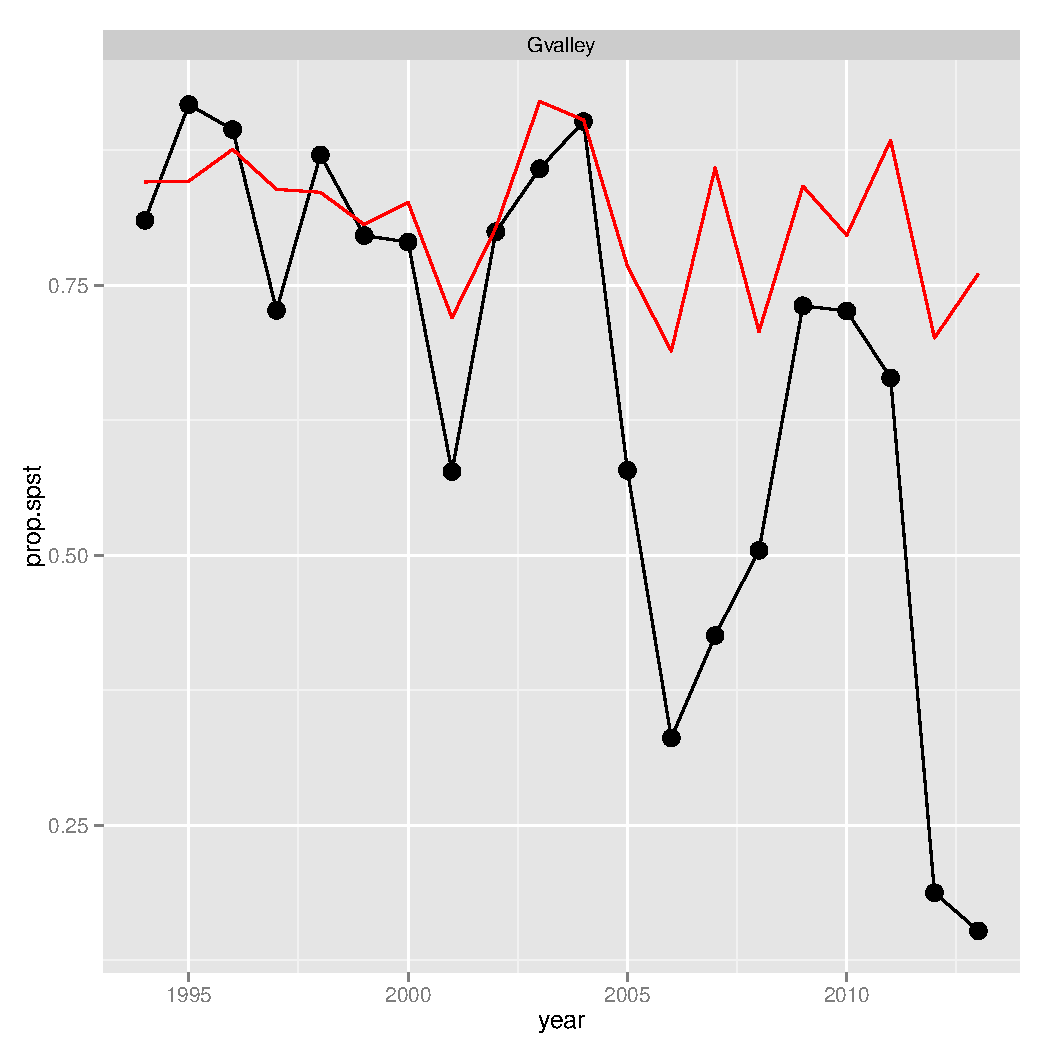
\includegraphics[width=\maxwidth]{figure/rtab1} 

\end{knitrout}

\caption{Example plot for tabset 1 \label{tab1}}
\end{figure}
As an example, we show here the proportion of Aedes.Vexan on Green Valley over time, the red line represents the average proportion of this species on each year. So on average across all years and sites, this species represents around 75\% of the mosquito counts. However on Green Valley the Aedes.Vexan proportion is most of the time below the mean, What happen in Green Valley ? The Vexans don't like it anymore !!!! 

\subsection{Tabset 2: Genotype-site}

In this tabset the user will find two checkedboxed, one to select the genotype (Aedes, Anopheles, Coquilletidia, Culex, Culiseta, Orthopodomyia, Psorophora and Uranotaenia ) and the other one to select the sites. In this case the user can select multiple sites and multiple genotypes. Here the idea is compare the genotypes in all the sites. After selcetion the user will see in each panel the proportion of a genotype in each year for a site or more than one.  The plot is faceted by genotype and each additional selected site will be added as a new line in the specific genotype plot.

The example shows the two most abundant genotypes in iowa mosquitos, Aedes and culex. 
\begin{figure}
\begin{knitrout}
\definecolor{shadecolor}{rgb}{0.969, 0.969, 0.969}\color{fgcolor}
\includegraphics[width=\maxwidth]{figure/rtab2} 

\end{knitrout}

\caption{Example plot for tabset 2 \label{tab2}}
\end{figure}

\subsection{Tabset 3: Location} 
In this tabset the user can select multiple species, after selection the user will see a plot with the Iowa map with the distributionof that specie in each site, the color indicate the abundance of the specific specie in the place. The idea in this tabset is see \textit{where} is more frequent to see a particular specie. The current dataset has only 8 sites and some species are not abundant a complete wite  map indicate the specie in the specific site does not like that place. If the color in the site is red then that specie is more abundat in that secific site. We can see the spacial distribution of the specie acros Iowa




\begin{figure}
\includegraphics[width=\textwidth]{mapaexample}
\caption{Example plot for tabset 3 \label{tab3}}
\end{figure}

\subsection{Tabset 4: Rare communities}
Besides describing each community we may be interesting in comparing them, in particular we want to know if all communities are alike or there are some site-year observations that are different from the rest. 
One important feature for the entomologist is to study the community characteristics, there are several indices reflecting different aspects of the mosquito community composition like abundance, simpson index, etc that will be useful for a community level comparison.

Working with species proportion within one site and year (instead of total counts) we compute an "average community" which simply taking average of each species proportion. 
Then for each observations we compute the distance respect to that average community. 

In this tabset the user will find  two select imputs with variables to describe the mosquito community composition and a scrol bar to select a specific quantile. After selection the user will see the density of the distance to the mean community, the red line is the quantile. In left panel each point is a site-year and the red ones are the extreme communities, the extreme values are colored based on the selected quantile (scrol bar) and in the axis we can select differenc variables to explain the community composition.  

We plot a two panel figure, on the right is the estimated density of the distances to the mid point community. The vertical red line represents the 90 quantile (as defect). 
\begin{figure}
\begin{knitrout}
\definecolor{shadecolor}{rgb}{0.969, 0.969, 0.969}\color{fgcolor}
\includegraphics[width=\maxwidth]{figure/rtab4} 

\end{knitrout}

\caption{Example plot for tabset 4 \label{tab4}}
\end{figure}

On the left panel there is a scatter plot of two community variables and we colored the points corresponding to communities further from the center community, this is with distance bigger than its 90\% quantile. 

On the shiny it is possible to choose the quantile that determine which communities are consider extreme and also the variables plot in the right panel. In this example the selected quantile is 90\% and the variables are Precipitation (horizontal) and Dominance index (vertical). Basically we can see all extreme communities shows big values in Dominance but are not extreme on precipitation. 

\subsection{Tabset MDS}
The last tabset presents also information at community level, this time we compute a distance matrix with every distances among each pair of communities. We an Multidimensional Scaling (MDS) to visualize the distance matrix, the distance computation and the MDS are done using {\tt vegan} package with {\tt vegdist} and {\tt metaMDS} functions. 

The user will see a scatterplot with the MDS results and going over any point with the mouse it will display some information to identify the specific community, in particular, information about site, year and distance from the center will be dispayed. 

Additionaly the user have the option to select a specific site and a specific year and will see these values colored and with different shape in the plot representation. 

\begin{figure}
\includegraphics[scale=.4, width=\textwidth]{screenshot}
\caption{Example plot for tabset 5 \label{tab5}}
\end{figure}

\subsection{Using the app}
We finish the web app description with a little intruction on how to run the application and get ready to analyze the mosquito surveillance data. You just need to follow these steps :

\begin{enumerate}
\item go to \href{https://github.com/nachalca/mosquito_shine}{https://github.com/nachalca/mosquito_shine}
\item copy the folder \textit{shiny$\_$msq} into your local machine
\item Open {\verb R } and change the working directory where \textit{shiny$\_$msq} folder is saved
\item run {\verb library(shiny) }
\item run {\verb runApp('shiny_msq') }
\end{enumerate}

\section{Computing}

There are 3 R files needed to run this app: {\verb ui.R }, {\verb server.R } and {\verb datasources.R }. The last one is a code read and transform the data set used by the shiny app. We describe the main characteristics of {\verb ui.R } and {\verb server.R } files in this section. 

\subsection{UI}

The ui have two principal aspects, the {\verb slidebarPanel } and {\verb mainPanel }, we have 5 tabsets in the web app and we design it to have differents shiny options on each tabset. Then the {\verb slidebarPanel } consist in a series of 5 {\verb conditionalPanel } one per tabset, for example the tabset 4 options are implemented by the following code

\begin{knitrout}
\definecolor{shadecolor}{rgb}{0.969, 0.969, 0.969}\color{fgcolor}\begin{kframe}
\begin{alltt}
          \hlkwd{conditionalPanel}\hlstd{(}\hlkwc{condition}\hlstd{=}\hlstr{"input.conditionedPanels==4"}\hlstd{,}
                           \hlkwd{img}\hlstd{(}\hlkwc{src}\hlstd{=}\hlstr{"Mosquito_da_Dengue_by_Lukemaciel.png"}\hlstd{,} \hlkwc{height} \hlstd{=} \hlnum{100}\hlstd{,} \hlkwc{width} \hlstd{=} \hlnum{300}\hlstd{),}
                           \hlkwd{sliderInput}\hlstd{(}\hlstr{"q"}\hlstd{,} \hlstr{"Quantile"}\hlstd{,}
                                       \hlkwc{min}\hlstd{=}\hlnum{0}\hlstd{,} \hlkwc{max}\hlstd{=}\hlnum{100}\hlstd{,} \hlkwc{value}\hlstd{=}\hlnum{90}\hlstd{,}\hlkwc{step}\hlstd{=}\hlnum{1}\hlstd{),}

                           \hlkwd{selectInput}\hlstd{(}\hlkwc{inputId} \hlstd{=} \hlstr{"index.X"}\hlstd{,}
                                      \hlkwc{label} \hlstd{=} \hlstr{"Select x axis variable"}\hlstd{,}
                                      \hlkwc{choices} \hlstd{= lab.index,}\hlkwc{selected}\hlstd{=}\hlstr{'PrecipationExact'}\hlstd{),}

                          \hlkwd{selectInput}\hlstd{(}\hlkwc{inputId} \hlstd{=} \hlstr{"index.Y"}\hlstd{,}
                                        \hlkwc{label} \hlstd{=} \hlstr{"Select y axis variable"}\hlstd{,}
                                        \hlkwc{choices} \hlstd{= lab.index,}\hlkwc{selected}\hlstd{=}\hlstr{'DegreeDayExact'}\hlstd{)}

           \hlstd{)}
\end{alltt}
\end{kframe}
\end{knitrout}


this create 3 options, the first one for selecting a quantile to act as a limit of what is consider as an extreme comunity, the other two allows the selection of the x and y variables for the scatterplot. 

The {\verb mainPanel } basically set up a tabpanel for each tabset we want to organize the output, the code is the following 
\begin{knitrout}
\definecolor{shadecolor}{rgb}{0.969, 0.969, 0.969}\color{fgcolor}\begin{kframe}
\begin{alltt}
    \hlkwd{mainPanel}\hlstd{(}
        \hlkwd{tabsetPanel}\hlstd{(}
            \hlkwd{tabPanel}\hlstd{(}\hlstr{"Species-site"}\hlstd{,}\hlkwd{p}\hlstd{(cap1),} \hlkwd{plotOutput}\hlstd{(}\hlstr{"plot1"}\hlstd{),}\hlkwd{tableOutput}\hlstd{(}\hlstr{"tab1"}\hlstd{),}\hlkwd{p}\hlstd{(cap1.1),}\hlkwc{value}\hlstd{=}\hlnum{1}\hlstd{),}

            \hlkwd{tabPanel}\hlstd{(}\hlstr{"Genotype-site"}\hlstd{,}\hlkwd{p}\hlstd{(cap6),} \hlkwd{plotOutput}\hlstd{(}\hlstr{"plot6"}\hlstd{),}\hlkwc{value}\hlstd{=}\hlnum{6}\hlstd{),}

            \hlkwd{tabPanel}\hlstd{(}\hlstr{"Location"}\hlstd{,} \hlkwd{plotOutput}\hlstd{(}\hlstr{"plot2"}\hlstd{),}\hlkwc{value}\hlstd{=}\hlnum{2}\hlstd{),}

            \hlkwd{tabPanel}\hlstd{(}\hlstr{"Indexes"}\hlstd{,} \hlkwd{plotOutput}\hlstd{(}\hlstr{"plot3"}\hlstd{),}\hlkwc{value}\hlstd{=}\hlnum{3}\hlstd{),}

            \hlkwd{tabPanel}\hlstd{(}\hlstr{"Rare Comunities"}\hlstd{,} \hlkwd{p}\hlstd{(cap4),}\hlkwd{plotOutput}\hlstd{(}\hlstr{"plot4"}\hlstd{),}\hlkwc{value}\hlstd{=}\hlnum{4}\hlstd{),}

            \hlkwd{tabPanel}\hlstd{(}\hlstr{"MDS"}\hlstd{,}\hlkwd{p}\hlstd{(cap5),} \hlkwd{ggvis_output}\hlstd{(}\hlstr{"my_plot"}\hlstd{),}\hlkwc{value}\hlstd{=}\hlnum{5}\hlstd{),}

            \hlkwc{id}\hlstd{=}\hlstr{"conditionedPanels"}\hlstd{)}

        \hlstd{)} \hlcom{# close mainPanel}
\end{alltt}
\end{kframe}
\end{knitrout}






\subsection{Server}

We have organized the server file in two main parts, a first part where we create reactive data set for each plot we want to include, and after using each reactive data set we create a reactive plot or table to include in the tabset. 

As an example, here is the dataset and the plot to create the last tabset, 

\begin{knitrout}
\definecolor{shadecolor}{rgb}{0.969, 0.969, 0.969}\color{fgcolor}\begin{kframe}
\begin{alltt}
\hlcom{# data for plot 5}
\hlstd{d5} \hlkwb{<-} \hlkwd{reactive}\hlstd{(\{}
    \hlkwd{data.frame}\hlstd{(mds2,} \hlkwc{sitecol} \hlstd{=} \hlkwd{as.factor}\hlstd{(mds2}\hlopt{$}\hlstd{site} \hlopt{==} \hlstd{input}\hlopt{$}\hlstd{site5),} \hlkwc{yearcol} \hlstd{=} \hlkwd{as.factor}\hlstd{(mds2}\hlopt{$}\hlstd{year} \hlopt{==}
        \hlstd{input}\hlopt{$}\hlstd{year5))}
\hlstd{\})}

\hlcom{# function for display information with the tooltip}
\hlstd{showSite} \hlkwb{<-} \hlkwa{function}\hlstd{(}\hlkwc{x}\hlstd{) \{}
    \hlkwa{if} \hlstd{(}\hlkwd{is.null}\hlstd{(x))}
        \hlkwd{return}\hlstd{(}\hlkwa{NULL}\hlstd{)}
    \hlstd{xx} \hlkwb{<-} \hlkwd{as.numeric}\hlstd{(x)}
    \hlstd{xx} \hlkwb{<-} \hlkwd{round}\hlstd{(xx,} \hlnum{4}\hlstd{)}
    \hlstd{ss} \hlkwb{<-} \hlstd{mds2[}\hlkwd{round}\hlstd{(mds2}\hlopt{$}\hlstd{MDS1,} \hlnum{4}\hlstd{)} \hlopt{==} \hlstd{xx[}\hlnum{1}\hlstd{]} \hlopt{&} \hlkwd{round}\hlstd{(mds2}\hlopt{$}\hlstd{MDS2,} \hlnum{4}\hlstd{)} \hlopt{==} \hlstd{xx[}\hlnum{2}\hlstd{],}
        \hlstd{]}
    \hlkwd{paste0}\hlstd{(}\hlstr{"<b>"}\hlstd{,} \hlstr{"Site:"}\hlstd{, ss}\hlopt{$}\hlstd{site,} \hlstr{"</b><br>"}\hlstd{,} \hlstr{"Year:"}\hlstd{, ss}\hlopt{$}\hlstd{year,} \hlstr{"<br>"}\hlstd{,} \hlstr{"Distance:"}\hlstd{,}
        \hlkwd{round}\hlstd{(ss}\hlopt{$}\hlstd{dist,} \hlnum{3}\hlstd{))}
\hlstd{\}}

\hlcom{# ggvis plot}
\hlstd{gv} \hlkwb{<-} \hlkwd{reactive}\hlstd{(\{}
    \hlcom{# check<-input_select(unique((mds2$site)))}
    \hlstd{p} \hlkwb{<-} \hlkwd{ggvis}\hlstd{(}\hlkwd{d5}\hlstd{(),} \hlkwd{props}\hlstd{(}\hlopt{~}\hlstd{MDS1,} \hlopt{~}\hlstd{MDS2,} \hlkwc{shape} \hlstd{=} \hlopt{~}\hlstd{yearcol,} \hlkwc{fill} \hlstd{=} \hlopt{~}\hlstd{sitecol,}
        \hlkwd{`:=`}\hlstd{(fill.hover,} \hlstr{"red"}\hlstd{),} \hlkwd{`:=`}\hlstd{(size.hover,} \hlnum{200}\hlstd{)))}
    \hlstd{p} \hlopt{+} \hlkwd{layer_point}\hlstd{()} \hlopt{+} \hlkwd{tooltip}\hlstd{(showSite)}
\hlstd{\})}

\hlcom{# set up the output plot}
\hlstd{output}\hlopt{$}\hlstd{controls} \hlkwb{<-} \hlkwd{renderControls}\hlstd{(gv)}
\hlkwd{observe_ggvis}\hlstd{(gv,} \hlstr{"my_plot"}\hlstd{, session)}
\hlstd{output}\hlopt{$}\hlstd{plot6} \hlkwb{<-} \hlkwd{reactivePlot}\hlstd{(}\hlkwa{function}\hlstd{() \{}
    \hlkwd{print}\hlstd{(}\hlkwd{ggplot}\hlstd{(}\hlkwc{data} \hlstd{=} \hlkwd{d6}\hlstd{(),} \hlkwd{aes}\hlstd{(}\hlkwc{x} \hlstd{= year,} \hlkwc{y} \hlstd{= prop.geno))} \hlopt{+} \hlkwd{geom_point}\hlstd{(}\hlkwc{size} \hlstd{=} \hlnum{2}\hlstd{)} \hlopt{+}
        \hlkwd{geom_line}\hlstd{(}\hlkwd{aes}\hlstd{(}\hlkwc{color} \hlstd{= site))} \hlopt{+} \hlkwd{facet_wrap}\hlstd{(}\hlkwc{facets} \hlstd{=} \hlopt{~}\hlstd{geno)} \hlopt{+} \hlkwd{scale_x_continuous}\hlstd{(}\hlstr{"Year"}\hlstd{)} \hlopt{+}
        \hlkwd{scale_y_continuous}\hlstd{(}\hlstr{"Proportion of geno"}\hlstd{))}
\hlstd{\})}
\end{alltt}
\end{kframe}
\end{knitrout}




\end{document}
